\subsection{Data-Flow Diagram (DFD)}
\label{subsec:dfd}
In this section the DFD of the alamAPI, specifically the Stock 
Market Price Trend Forecasting System will be presented and discussed. 
A data-flow diagram will help to better understand how the processes works, 
and how data flows from one process to another. This is specifically important 
as it shows the overview of the security of the data by showing how it can be 
accessed. In the case of alamAPI, the data that can only be accessed publicly is 
the listed stock to buy and sell, as well as the stock information as provided 
in its database, and as allowed by the API endpoints.
\hfill \\

Moreover, the DFD paradigm used in the diagrams presented in this 
section follows the Gane-Sarson DFD symbols, which utilizes four basic symbols: 
(1) Entity / External Entity; 
(2) Data Flow; 
(3) Process; and 
(4) Data Store 
\cite{VisualParadigm}
% Context Diagram
\subsubsection{Context Diagram}
\label{subsubsec:context_dfd}
First, let us start by showing the overview of 
the whole process by showing the context diagram of the system itself as 
process 0, which can be seen in the provided in Figure \ref{fig:context_dfd}.
\begin{figure}[ht]
    \centering
    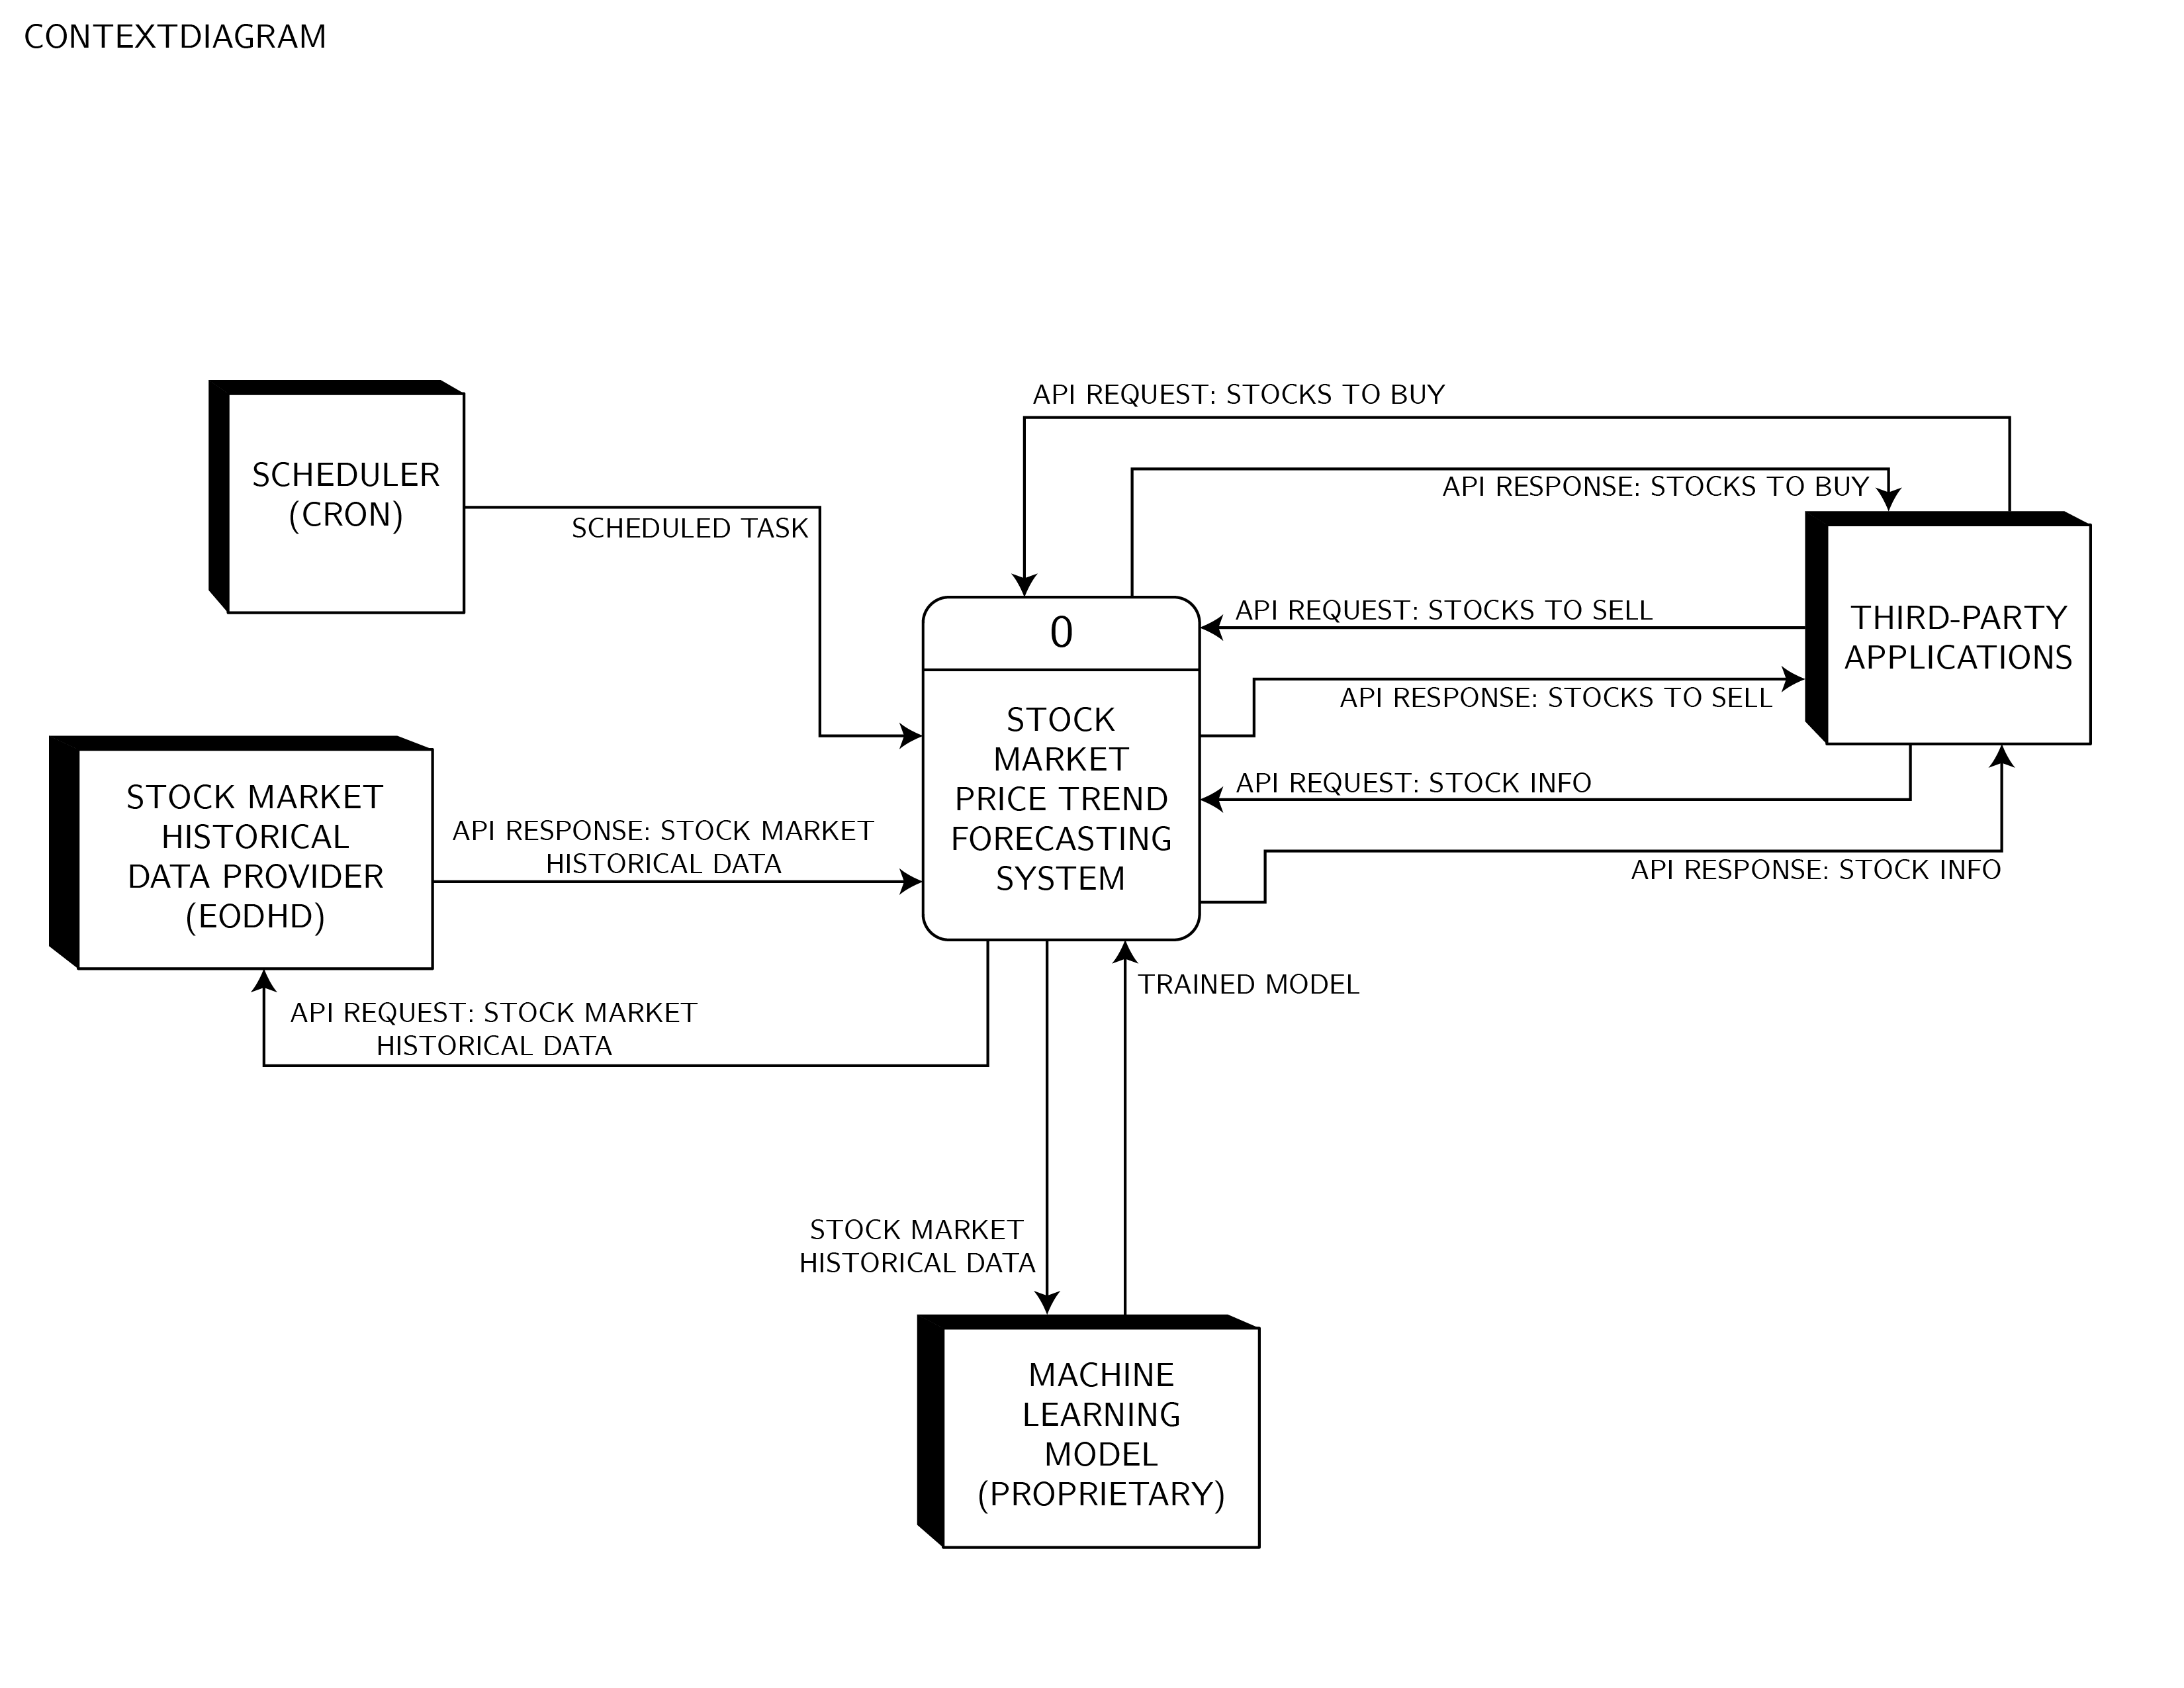
\includegraphics[width=1\textwidth]{./assets/Data Flow Diagram-01.png}
    \caption{Context Diagram of the Stock Market Price Trend Forecasting System}
    \label{fig:context_dfd}
\end{figure}
\FloatBarrier
\vspace{0.5cm}
The above figure shows the root process (process 0), which is the underlying 
system of the alamAPI itself: Stock Market Price Trend Forecasting (SMPTF) 
System which is connected to four external entities: (1) Scheduler, 
which will be provided by CRON; (2) Stock Market Historical Data Provider, 
which will be EODHD; (3) Machine Learning Model, which will be developed 
along side the development of the system; and (4) Third-Party Application, 
which will also be developed in the conduct of this special problem as the 
test application for accessing, testing, and showcase of the features of alamAPI.
\hfill \\

Moreover, all the necessary data flow lines can also be observed: 
(1) Scheduled task, which is the committed task on schedule as indicated 
in the CRON application; 
(2) API Request: Stock Market Historical Data, which is the request 
information passed by the root process to the historical market data provider; 
(3) API Response: Stock Market Historical Data, which is the data passed by the 
historical market data provider to the process after accepting its request; 
(4) Trained Model, this is the object class from the Machine Learning model that 
will be developed and used by the system; 
(5) Stock Market Historical Data, as the name suggests this is the historical 
market data which will also be used to train and improve the machine learning model; 
(6) API Request: Stocks to Buy, which is the data passed from the third-party 
application to the root process to request for which stocks are in the Buy 
document of the database; 
(7) API Response: Stocks to Buy, upon the request of the third-party application, 
the root process will process the request to the API and sends back the 
list of stocks to buy to the requester; 
(8) API Request: Stocks to Sell, which is the data passed from the 
third-party application to the root process to request for which stocks 
are in the Sell document of the database; 
(9) API Response: Stocks to Sell, upon the request of the third-party application, 
the root process will process the request to the API and sends back the list of 
stocks to sell to the requester; 
(10) API Request: Stock Info, which is the data passed from the third-party 
application to the root process to request for the general information about a 
particular stock, this will be further discussed in the Object-Document Mapped 
(ODM) diagram; and 
(11) API Response: Stock Info, upon the request of the third-party application, 
the root process will process the request to the API and sends back the information 
of the stock based on what was requested.

% DFD 0
\subsubsection{DFD of Diagram 0}
\label{subsubsec:dfd0}
To better understand how each data going in-and-out 
of the root process, is being processed, it is essential that we look inside 
the inner workings of the root process, which is shown in the DFD of Diagram 0, 
as provided in Figure \ref{fig:dfd0}.
\begin{figure}[ht]
    \centering
    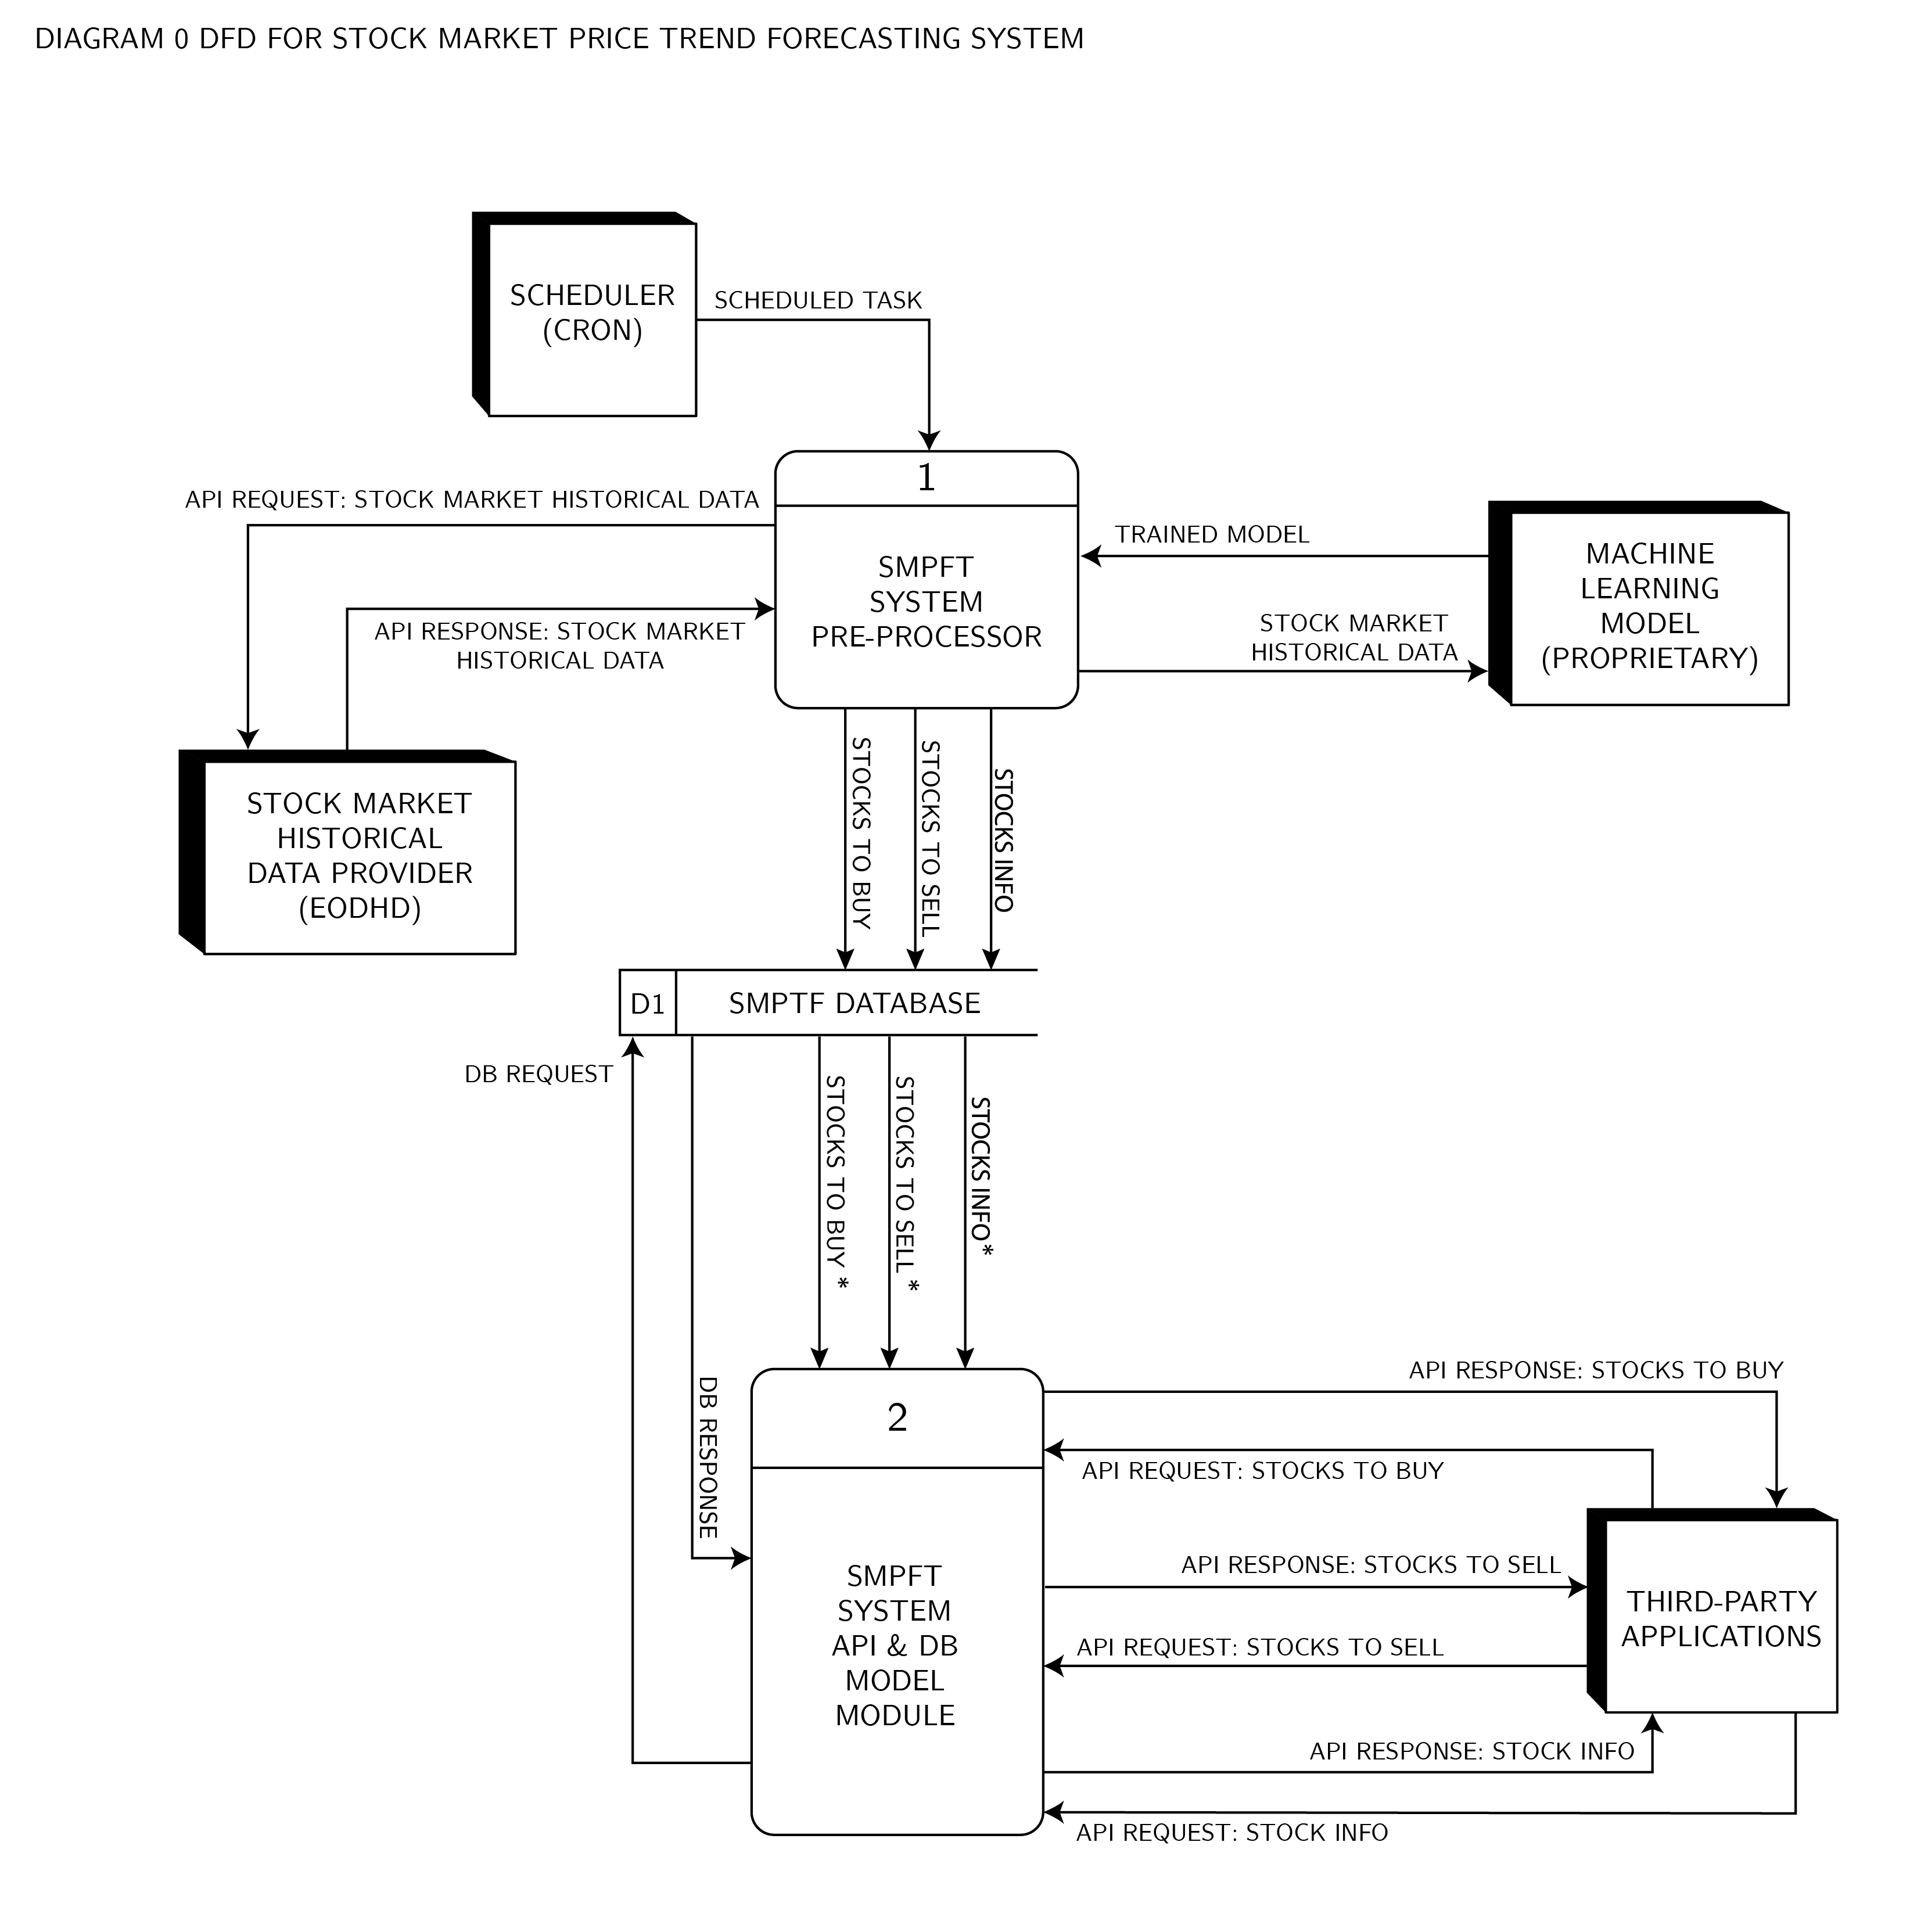
\includegraphics[width=1\textwidth]{./assets//Data Flow Diagram-02.png}
    \caption{DFD of Diagram 0}
    \label{fig:dfd0}
\end{figure}
\FloatBarrier

From the figure above, the root process, has two main processes: 
(1) SMPFT System Pre-Processor, which is the system’s data processing unit; and 
(2) SMPFT System API and DB Model Module, which processes the API 
requests and responses, as well as the database of the system.

% DFD 1
\subsubsection{DFD of Diagram 1}
\label{subsubsec:dfd1}
To better understand the internal workings of the 
Process 1, it will be useful to check the DFD of that process, 
which is provided in Figure \ref{fig:dfd1}
\begin{figure}[ht]
    \centering
    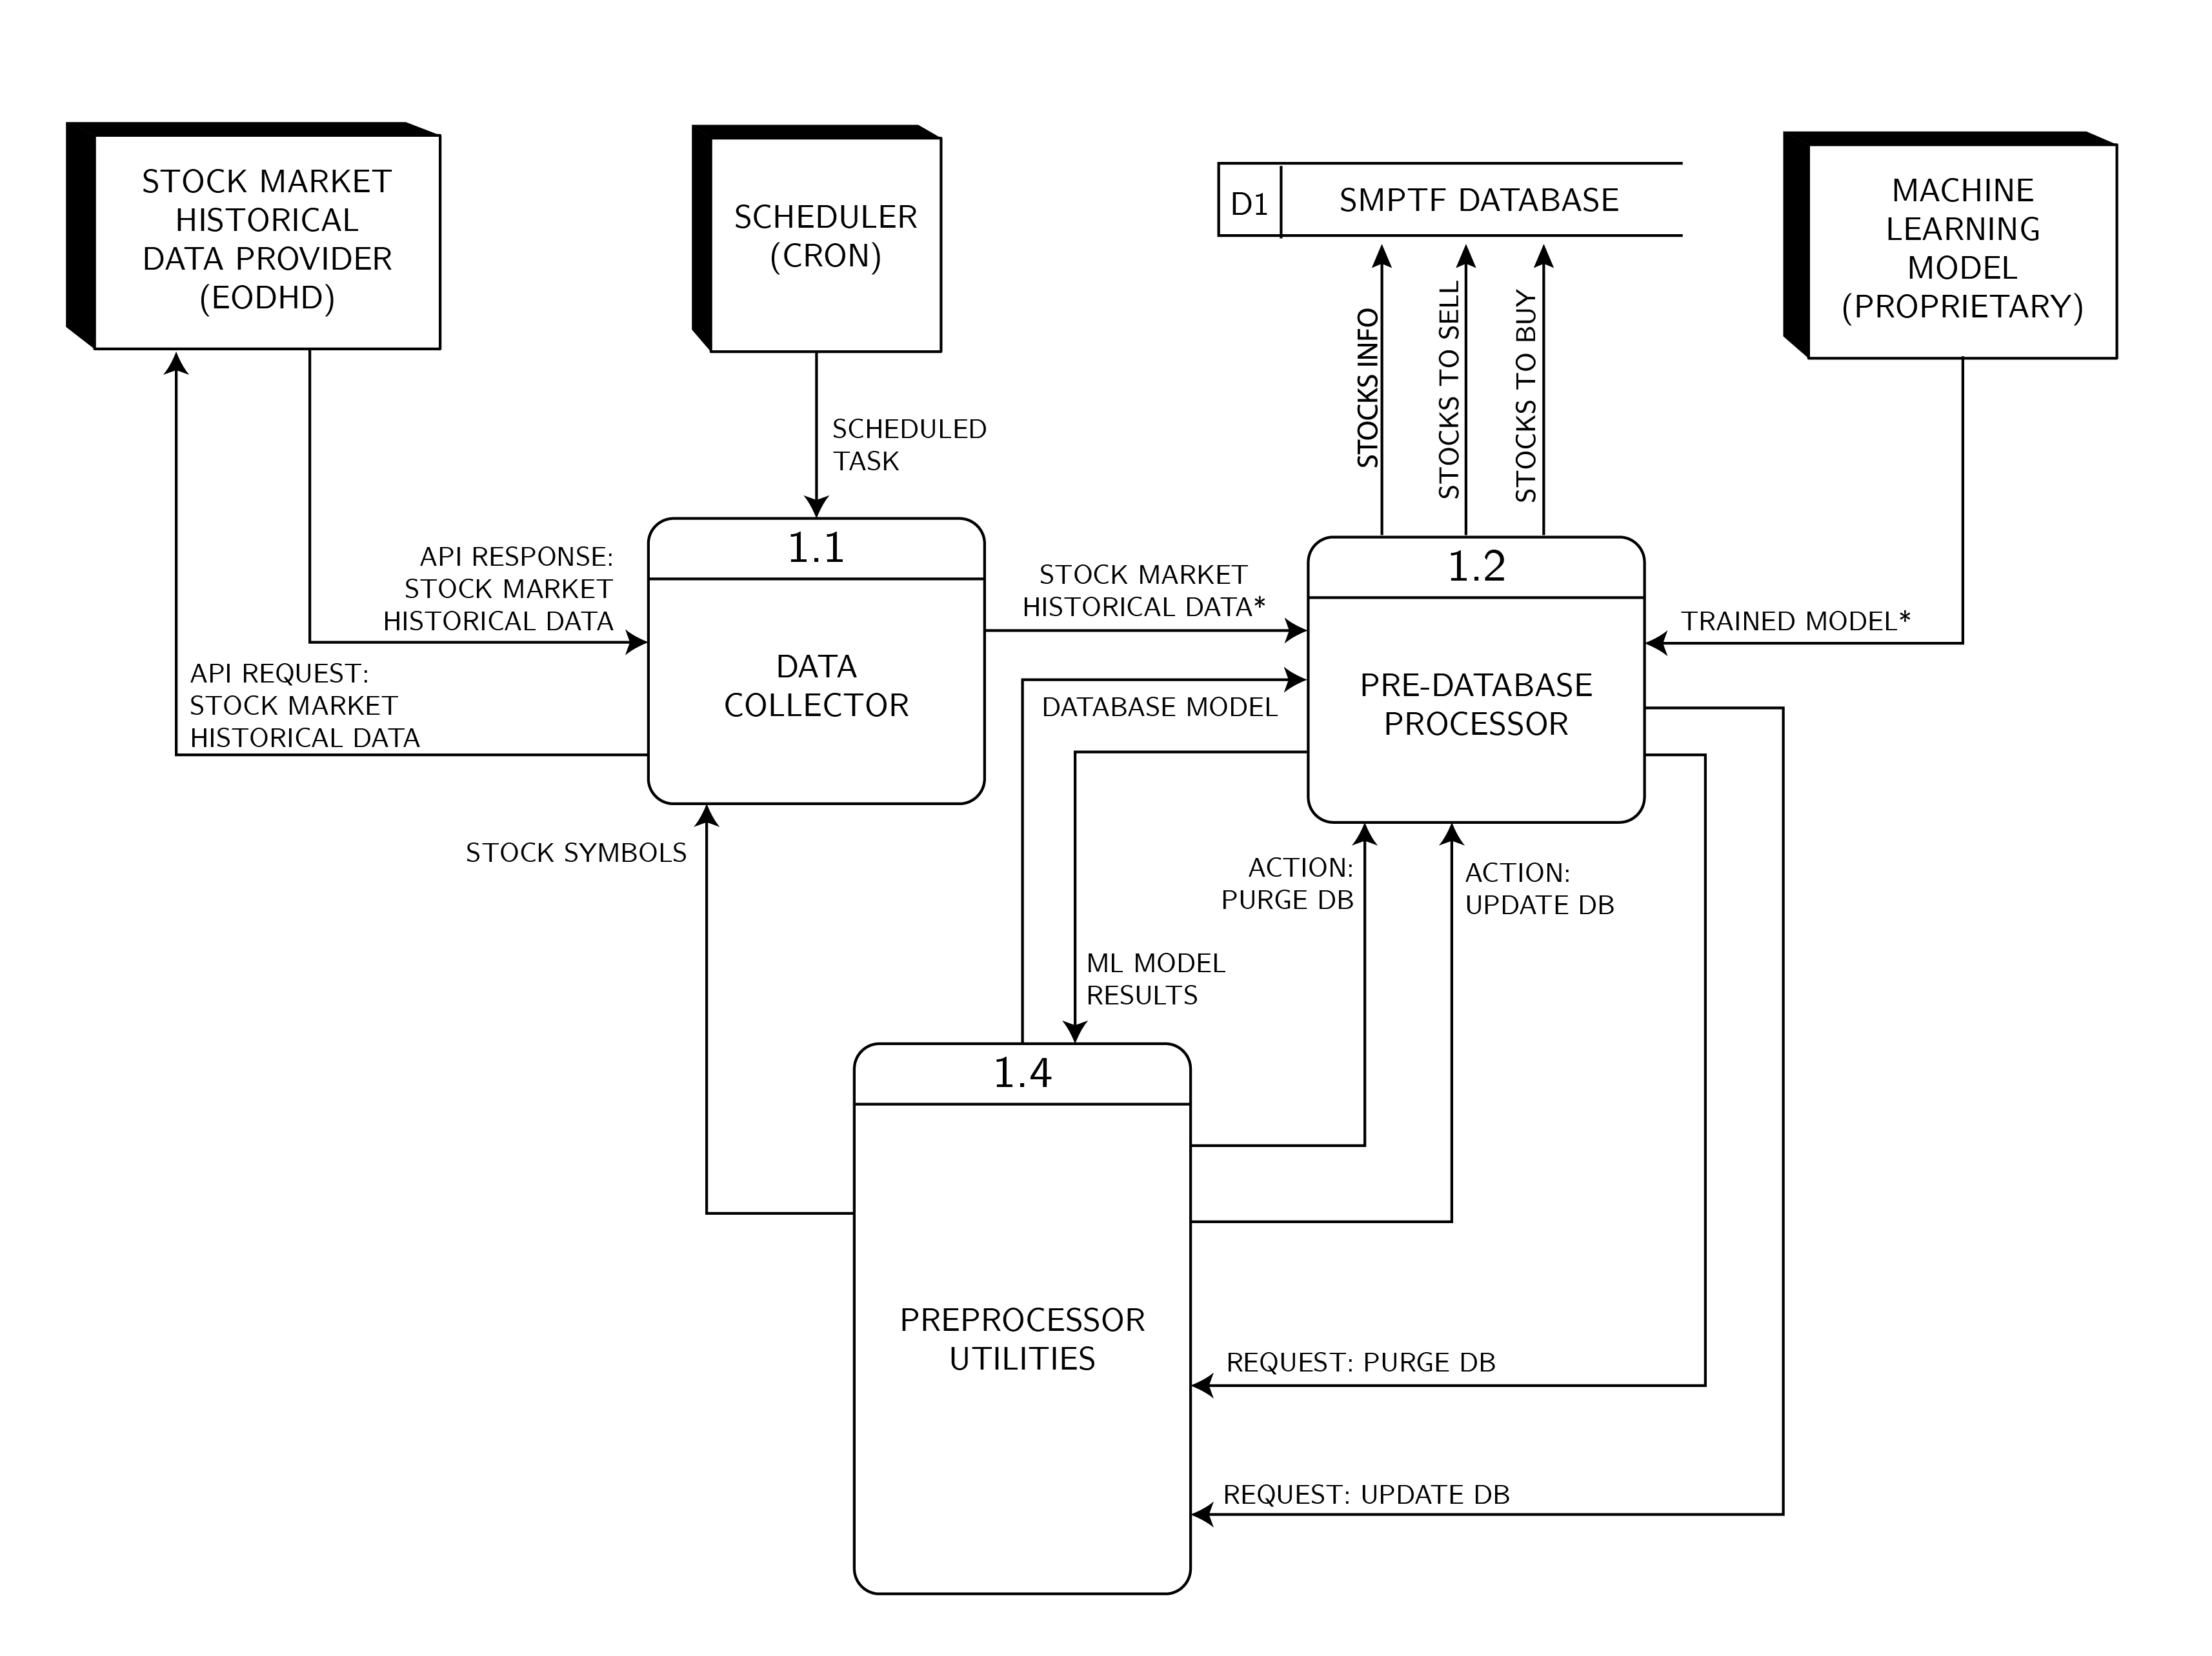
\includegraphics[width=1\textwidth]{./assets/Data Flow Diagram-03.png}
    \caption{DFD of Diagram 1}
    \label{fig:dfd1}
\end{figure}
\FloatBarrier

From the figure shown above, it can be observed that Process 1 
is composed of 4 internal processes, namely, 
(1) Data Collector, which is the main process responsible 
for collecting the historical market data; 
(2) Pre-Database Processor, which is the processes that the collected 
data goes into before being sent to the system’s database, the 
internal processes of this process will be further discuss in the 
succeeding part of this section; 
(3) Machine Learning Model Processor, which is the training module or 
process for the machine learning model that is used to externally train 
the machine learning model that will be used by the system in the 
pre-database processor; and 
(4) Preprocessor Utilities, this will be the processes the process any 
system utilities such as the database actions, database models, and 
stores temporary data and system variables.

% DFD 1.2
\subsubsection{DFD of Diagram 1.2}
\label{subsubsec: dfd1.2}
This shows the processes inside the process 1.2: 
Pre-database Processor.
\begin{figure}[ht]
    \centering
    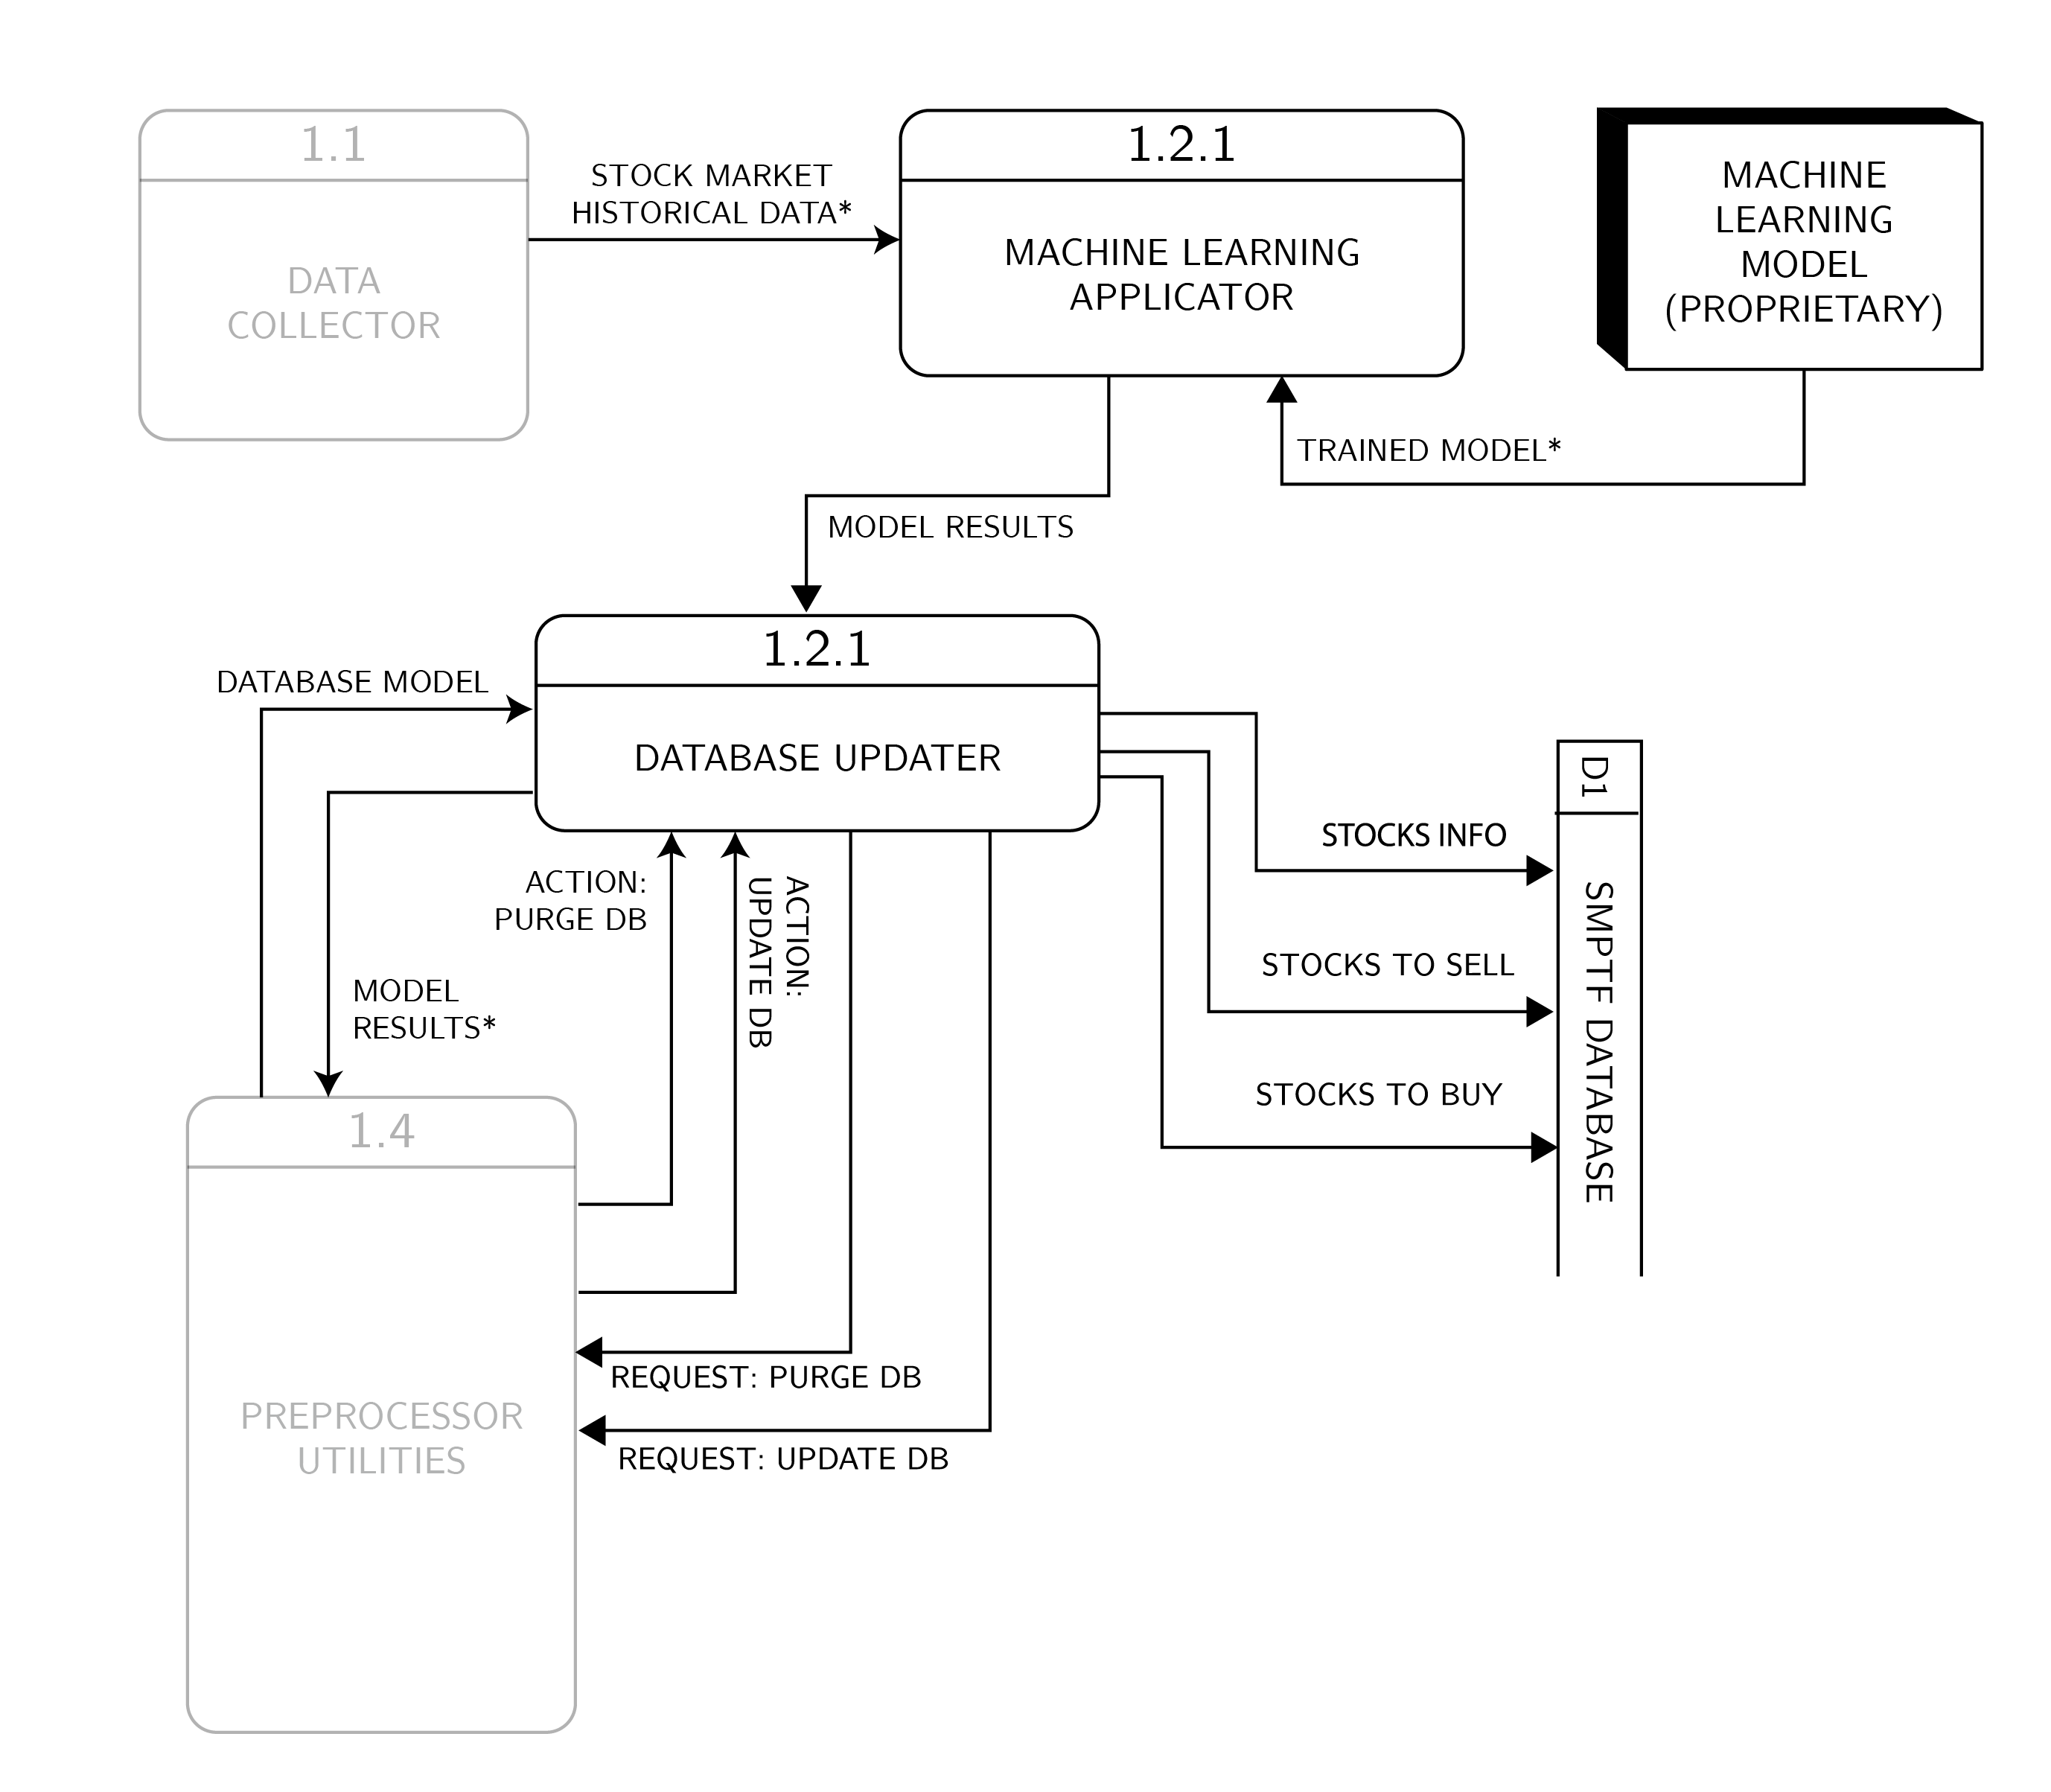
\includegraphics[width=1\textwidth]{./assets/Data Flow Diagram-05.png}
    \caption{DFD of Diagram 1.2}
    \label{fig:dfd1.2}
\end{figure}
\FloatBarrier

As previously discussed, the pre-database processor consists of processes 
inside that processes the data before it will be eventually sent to the database 
of the system. Wherein the process and data flow is shown in the figure above. 
Namely: (1) Machine Learning Applicator, which applies the trained machine learning 
model to the collected data; and 
(2) Database Updater, which processes the document outputs from the Machine 
Learning Applicator process, to be used in the database of the system.


% DFD 2
\subsubsection{DFD of Diagram 2}
\label{subsubsec:dfd2}
The final diagram will show the inner processes of 
the Process 2: SMPFT System API and DB Model Module.
\begin{figure}[ht]
    \centering
    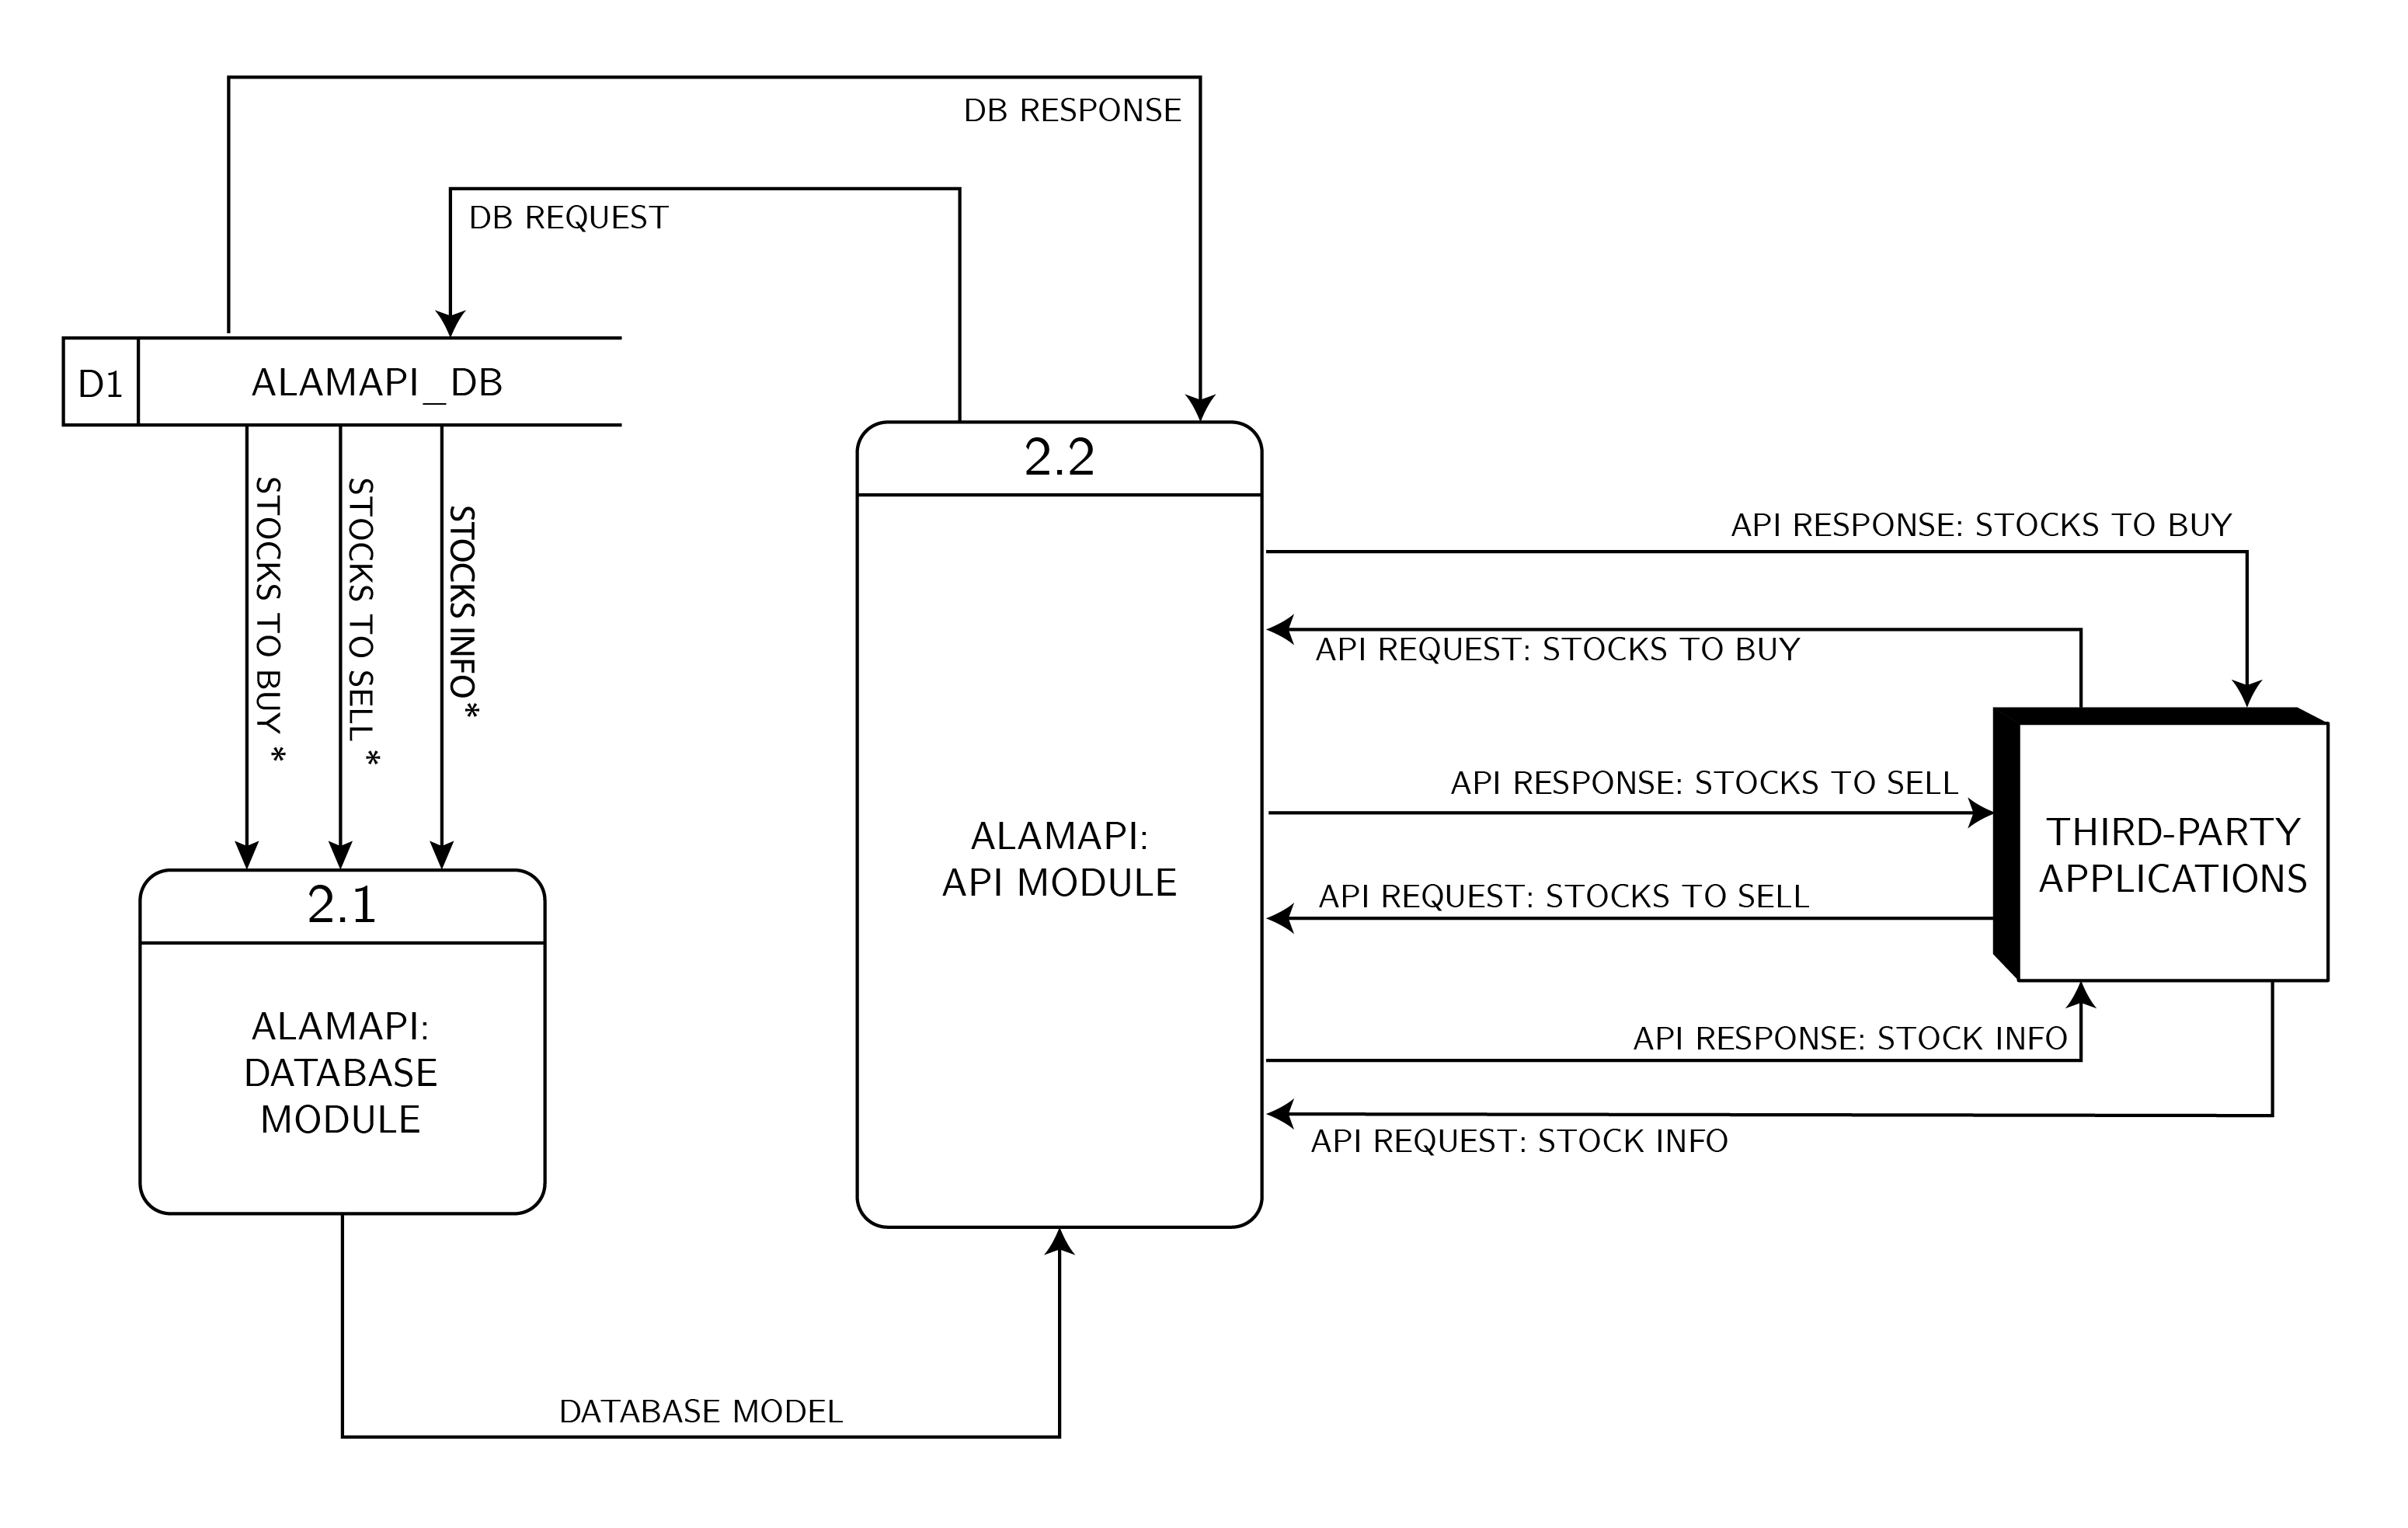
\includegraphics[width=1\textwidth]{./assets/Data Flow Diagram-04.png}
    \caption{DFD 2: Data-Flow Diagram for the alamAPI}
    \label{fig:dfd2}
\end{figure}
\FloatBarrier
\vspace{0.5cm}
The figure above shows two internal processes of the Process 2, namely, 
(1) SMPFT DB Model, which the database model that is used to process and 
connect MongoDB to the Python program; and 
(2) SMPFT API, which is composed of the API endpoints that processes 
the requests and response to and from the system, respectively.